\chapter{Results}\label{chapter:5}

{\color{red}Utilizing the methods described in the previous chapters, we present numerical results consistent with singularity formation in the Euler flow starting from $\be_{TGV}$, $\be_S$ and $\be_L$. However, to obtain these results we must extend the time interval to $T=25$. We also present numerical results that a singularity does form in the Euler flow corresponding to the optimal initial conditions $\tilde{\be}_{8,3}$ and $\tilde{\be}_{8,5}$, within the corresponding time intervals, using $\be_{TGV}$ as the initial guess. Additionally, our numerical results indicate that a singularity does not form in the flow corresponding to the optimal initial conditions $\tilde{\be}_{8,3}$ or $\tilde{\be}_{8,5}$ within the corresponding time intervals, using $\be_S$ as the initial guess. However, by starting from $\tilde{\be}_{8,5}$ and evolving the solution over the time interval $T=25$, we obtain results consistent with singularity formation in the Euler flow. Finally, we present numerical evidence that a singularity DOES(NT) form in the Euler flow corresponding to the optimal initial conditions $\be_{8,3}$ or $\be_{8,5}$, using $\be_L$ as the initial guess.}

\section{Singularity Detection}

Theorem \ref{thm:Theorem:1.3} provides the criteria we use to determine if a singularity forms in the Euler flow corresponding to initial condition $\be$, where $\be$ is the optimal initial condition found in the limit $\alpha\rightarrow 0$ by solving Problem \ref{eq:problem} as described in Chapter \ref{chapter:3}. In practice, we take $\be$ to be the optimal initial condition found for the smallest value of $\alpha$ for which the calculations were well resolved, i.e, $\tilde{\be}_{8,T}$. First, we check if the sequence of optimal initial conditions, found by solving Problem \ref{eq:problem} for decreasing $\alpha$, converges to a well-defined limit, i.e, if they satisfy (\ref{eq:eta:0:condition}). If this condition is satisfied, we then check whether (\ref{eq:alpha:sup}) is satisfied and $\alpha^2\pat$ converges to a positive limit as $\alpha\rightarrow 0$. 
\\~\\
Simply plotting the left-hand side (LHS) in (\ref{eq:eta:0:condition}) and (\ref{eq:alpha:sup}) as functions of $\alpha$ will not be sufficient for determining if each condition is satisfied. This is due to the fact that it is difficult to detect if these expressions are converging to zero or to some small positive limit. In order to make this determination we use the method of \cite{larios_computational_2018}, which proposes the following ansatz,
\begin{equation}\label{eq:ansatz:1}
\sup_{t\in[0,T]}\|\nabla\ua(t)\|_{L^2} \approx \mathcal{O}(\alpha^p),
\end{equation}
for $T > 0$ sufficiently large and for some power $p$. From this and Theorem \ref{thm:Theorem:1.3}, in order for a singularity to form in the Euler flow, it must be the case that the increase in the objective functional offsets the decrease of $\alpha$, which can only occur if $p\leq -1$. However, if $p<-1$, then the gradient term in (\ref{eq:alpha:Energy}) will become unbounded as $\alpha\rightarrow 0$. This would mean the $\alpha$-energy is not conserved. Therefore, for a singularity to form, it must be the case that strictly $p = -1$. To find the value of $p$, we create a log-log plot of $\text{max}_{t\in[0,T^*]}\|\bn \ua(t)\|_{L^2}$ vs $\alpha$. In order to simplify the visualization of the evolution of this quantity over time, the figures included here will only include the results at $t=0,1,...,T$. The value of $p$ is defined as the steepest slope between any two values of $\alpha$ at any point in the time window.
\\~\\
We utilize the same method to determine if (\ref{eq:eta:0:condition}) is satisfied. However, in this case the condition is satisfied if the quantity does converge to zero. The condition is a sum of a energy term, $\|\be-\bea\|_{L^2}^2$ and a enstrophy term, $\|\bn(\be-\bea)\|_{L^2}^2$, which is scaled by $\alpha^2$. From Poincare's inequality, if the enstrophy term diminishes to zero as $\alpha\rightarrow 0$, then so too does the energy term and so (\ref{eq:eta:0:condition}) is satisfied \cite{doering_applied_1995}. However, if the enstrophy term diverges, but does so more slowly than $\alpha$ diminishes, then (\ref{eq:eta:0:condition}) is only satisfied if the energy term also goes to zero with $\alpha$. Finally, if the enstrophy term diverges more quickly than $\alpha$ diminishes then (\ref{eq:eta:0:condition}) is not satisfied. Therefore, we propose the following two ansatze.
\begin{equation}\label{eq:ansatz:3}
\|\bn(\be-\bea)\|_{L^2} \approx \mathcal{O}(\alpha^q).
\end{equation}
and
\begin{equation}\label{eq:ansatz:2}
\|\be-\bea\|_{L^2} \approx \mathcal{O}(\alpha^r),
\end{equation}
By creating log-log plots of the LHS in (\ref{eq:ansatz:3}) and (\ref{eq:ansatz:2}) vs $\alpha$, the values of $q$ and $r$ are given by the steepest slope between any two values of $\alpha$ at any point in time for (\ref{eq:ansatz:3}) and (\ref{eq:ansatz:2}), respectively. For (\ref{eq:eta:0:condition}) to be satisfied, it must be the case that either $r>0$, or $-1<r\leq 0$ and $q>0$.

\section{Results Obtained Using the Initial Guesses}
{\color{red}
We begin by presenting our results obtained using the initial guesses, $\be_{TGV}$, $\be_S$, and $\be_L$. These serve as a baseline comparison with the results obtained by solving Problem \ref{eq:problem}. Without optimization, the initial conditions for all values of $\alpha$ are simply the initial guess. In this case, it is trivially true that condition (\ref{eq:eta:0:condition}) is satisfied, and so we only need to compute the value of $p$ to determine if a singularity forms in the Euler flow corresponding to the initial guess.

\subsection{Results Obtained Using $\be_{TGV}$}

A visualization of the vorticity of $\be_{TGV}$ is shown in Figure \ref{fig:TGV:Init}. Figure \ref{fig:T3:TGV:visual} shows the vorticity of $\omega = \bn \times \ua(T=3;\be_{TGV})$ for $\alpha=8/1024$ and Figure \ref{fig:T5:TGV:visual} shows the vorticity of $\omega = \bn \times \ua(T=5;\be_{TGV})$ for $\alpha=8/1024$. The figures show that the areas of high vorticity are concentrated into smaller area as the flow evolves and that the peak of the vorticity increases in magnitude.
\\~\\

\begin{figure}[h!]
\centering
\begin{subfigure}{.4\textwidth}
  \centering
  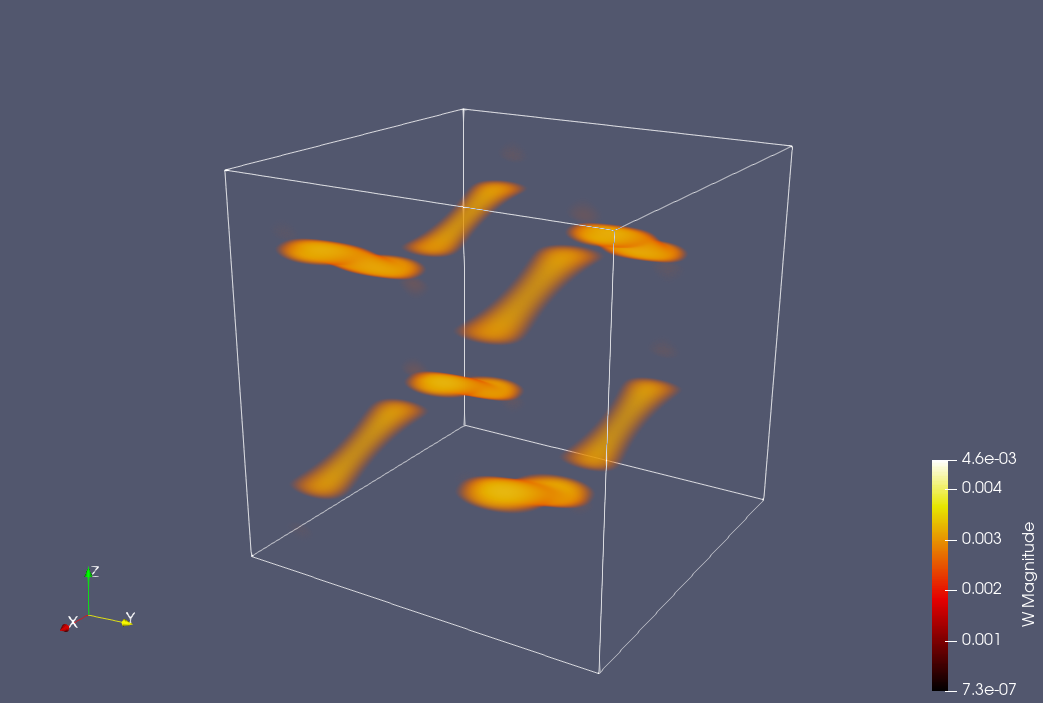
\includegraphics[width=.9\linewidth]{../../results/Final_Results/Visualizations/Nonoptimization_Results_T3/alpha_8_1024/Terminal_W_M_shifted.png}
  \caption{}
  \label{fig:sub1}
\end{subfigure}%
\begin{subfigure}{.4\textwidth}
  \centering
  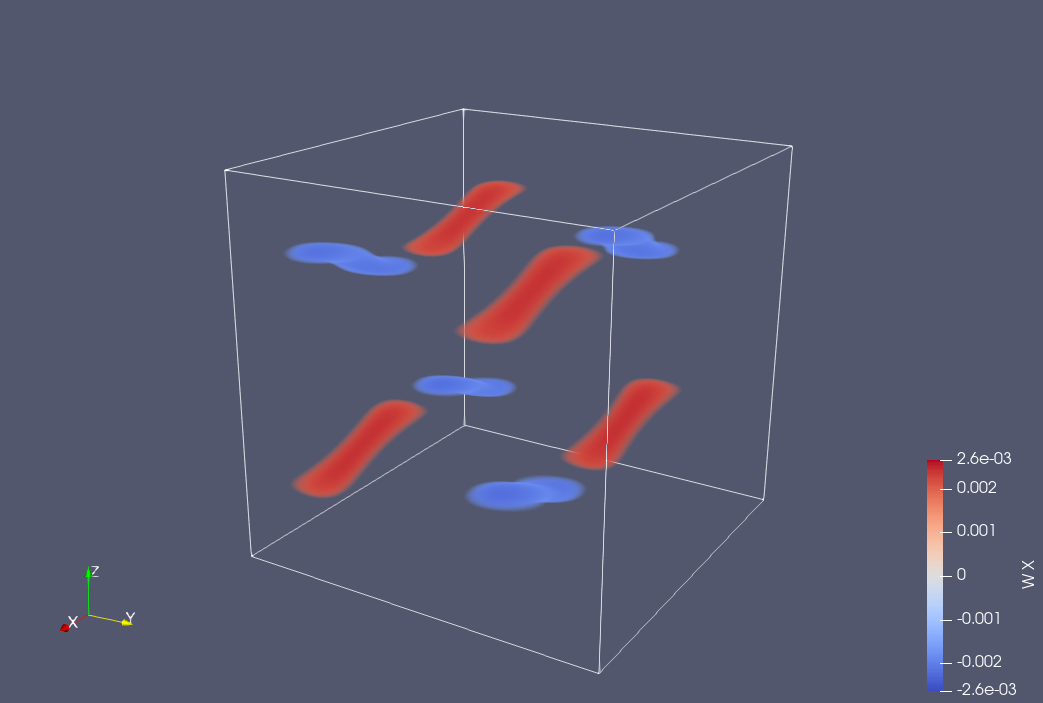
\includegraphics[width=.9\linewidth]{../../results/Final_Results/Visualizations/Nonoptimization_Results_T3/alpha_8_1024/Terminal_W_X_shifted.png}
  \caption{}
  \label{fig:sub2}
\end{subfigure}
\\
\begin{subfigure}{.4\textwidth}
  \centering
  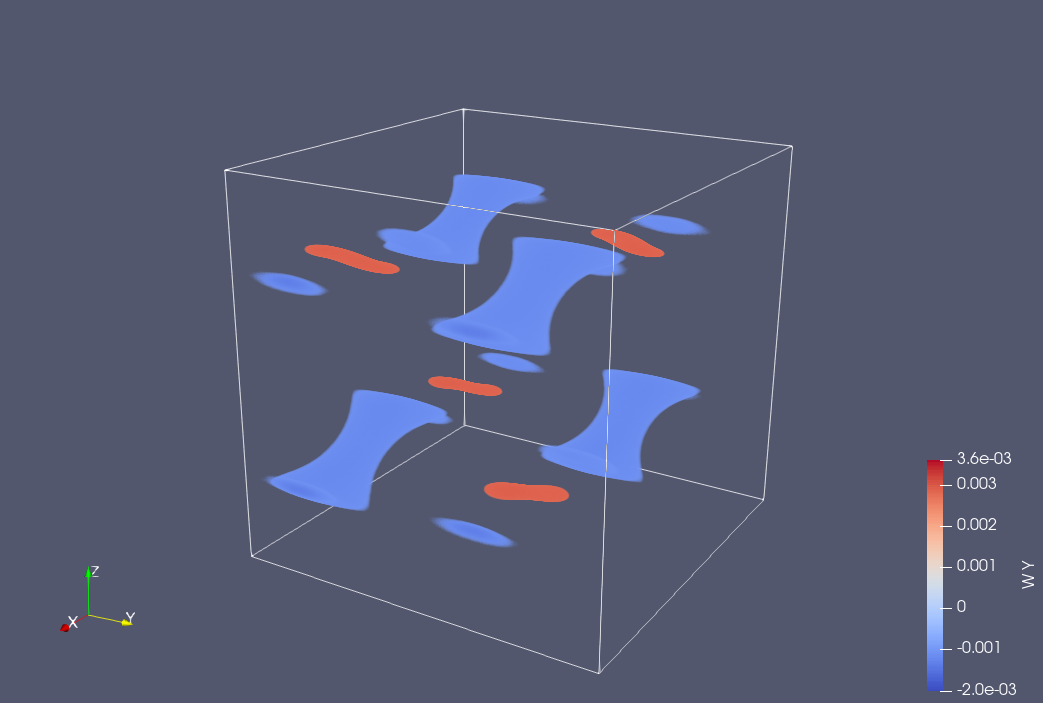
\includegraphics[width=.9\linewidth]{../../results/Final_Results/Visualizations/Nonoptimization_Results_T3/alpha_8_1024/Terminal_W_Y_shifted.png}
  \caption{}
  \label{fig:sub1}
\end{subfigure}%
\begin{subfigure}{.4\textwidth}
  \centering
  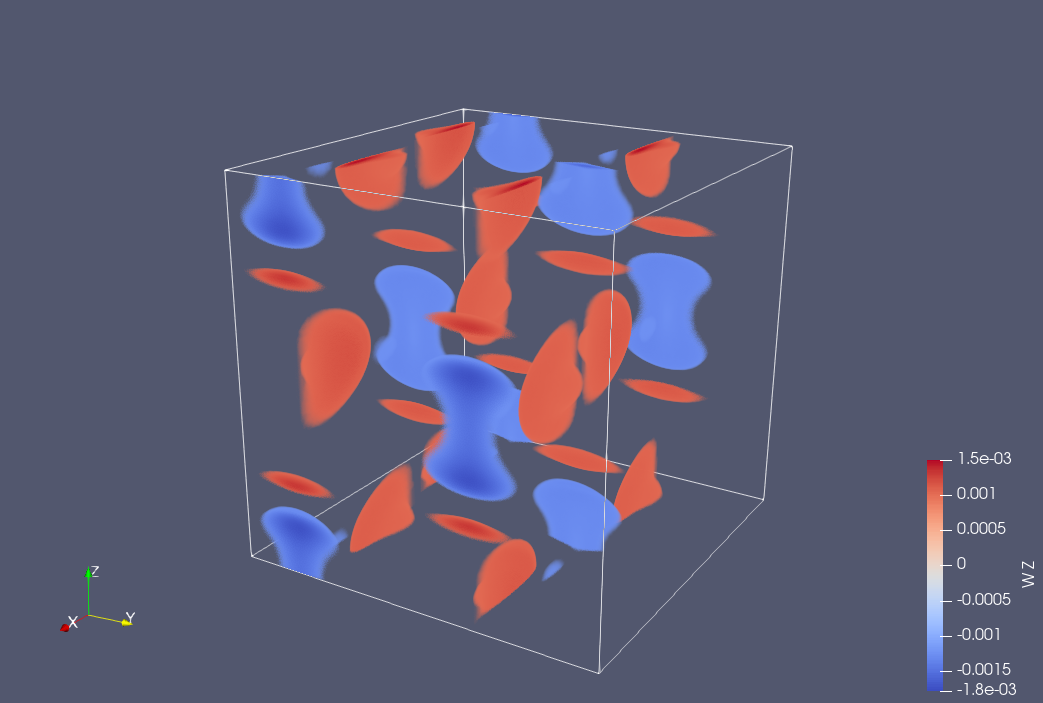
\includegraphics[width=.9\linewidth]{../../results/Final_Results/Visualizations/Nonoptimization_Results_T3/alpha_8_1024/Terminal_W_Z_shifted.png}
  \caption{}
  \label{fig:sub2}
\end{subfigure}
\caption{Isosurfaces of vorticity $\omega=\bn \times \ua(T=3;\be_{TGV})$ with $\alpha=8/1024$. (a) magnitude $|\w(\x)|$, and components (b) $|\omega_1|$, (c) $|\omega_2|$, and (d) $|\omega_3|$.}
\label{fig:T3:TGV:visual}
\end{figure}


\begin{figure}
\centering
\begin{subfigure}{.4\textwidth}
  \centering
  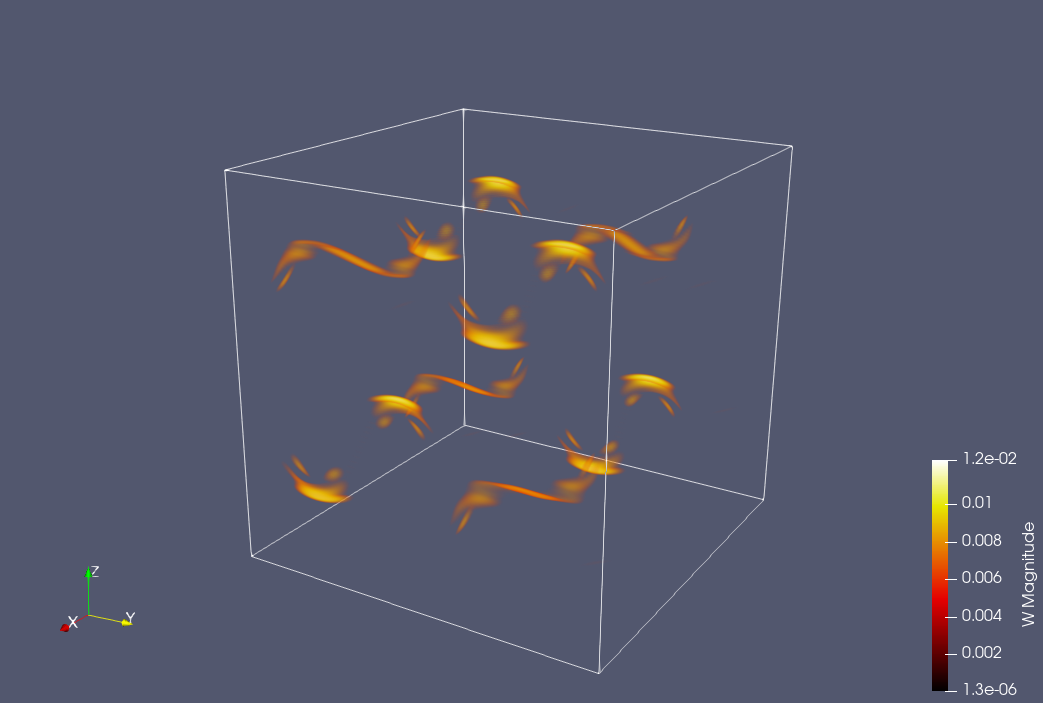
\includegraphics[width=.9\linewidth]{../../results/Final_Results/Visualizations/Nonoptimization_Results_T5/alpha_8_1024/Terminal_W_M_shifted.png}
  \caption{}
  \label{fig:sub1}
\end{subfigure}%
\begin{subfigure}{.4\textwidth}
  \centering
  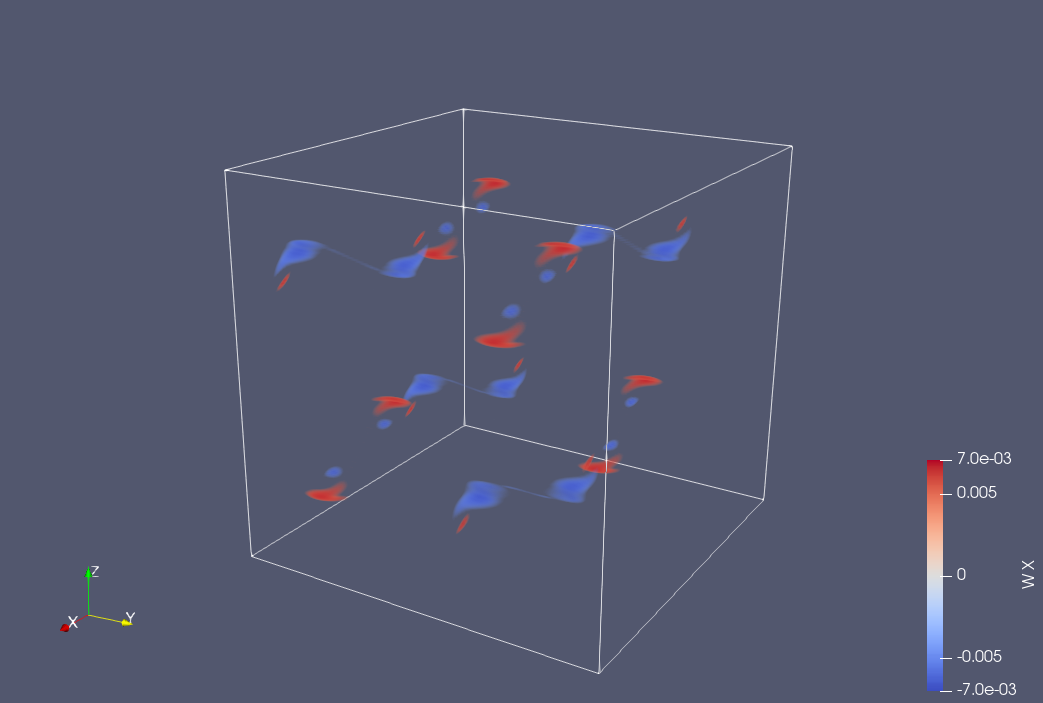
\includegraphics[width=.9\linewidth]{../../results/Final_Results/Visualizations/Nonoptimization_Results_T5/alpha_8_1024/Terminal_W_X_shifted.png}
  \caption{}
  \label{fig:sub2}
\end{subfigure}
\\
\begin{subfigure}{.4\textwidth}
  \centering
  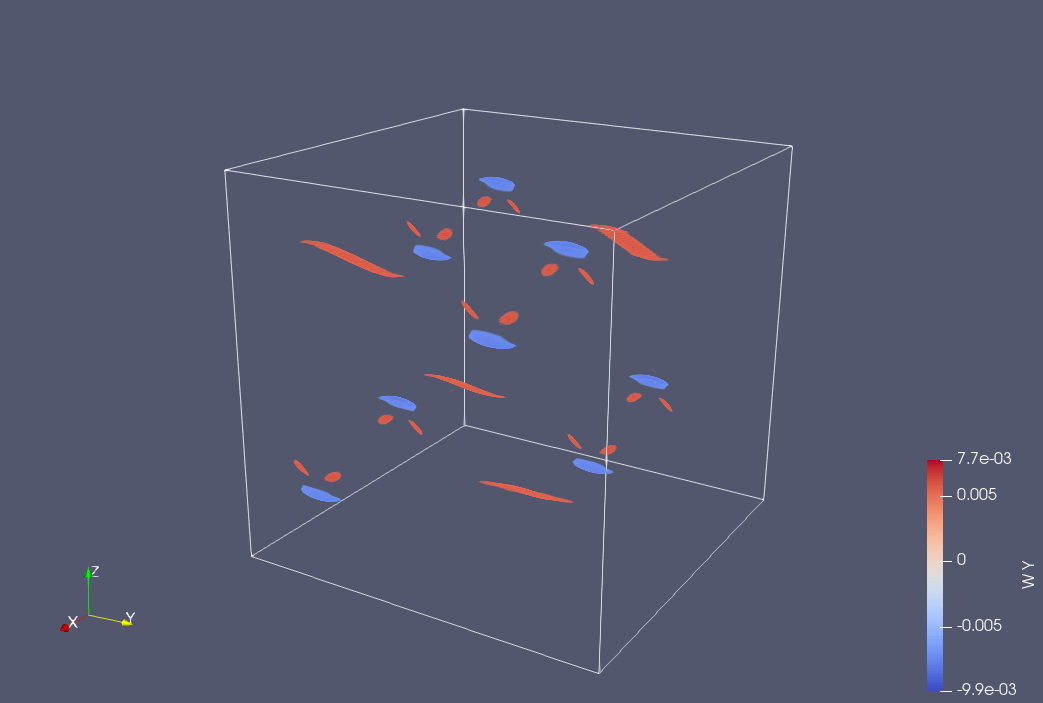
\includegraphics[width=.9\linewidth]{../../results/Final_Results/Visualizations/Nonoptimization_Results_T5/alpha_8_1024/Terminal_W_Y_shifted.png}
  \caption{}
  \label{fig:sub1}
\end{subfigure}%
\begin{subfigure}{.4\textwidth}
  \centering
  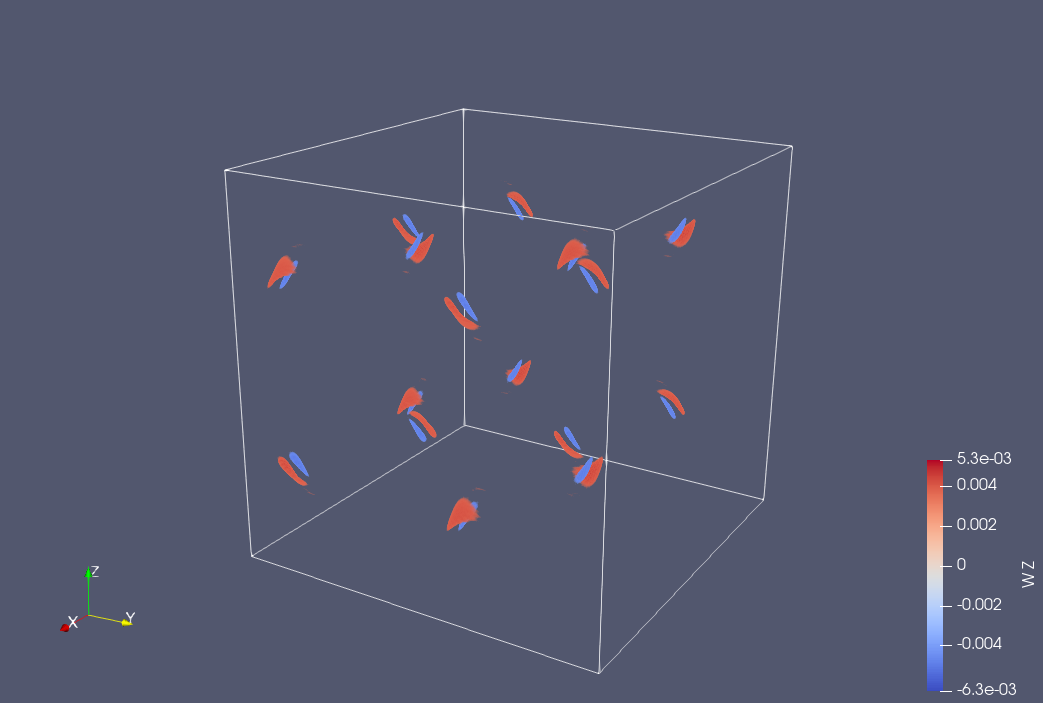
\includegraphics[width=.9\linewidth]{../../results/Final_Results/Visualizations/Nonoptimization_Results_T5/alpha_8_1024/Terminal_W_Z_shifted.png}
  \caption{}
  \label{fig:sub2}
\end{subfigure}
\caption{Isosurfaces of vorticity $\omega=\bn \times \ua(T=5;\be_{TGV})$ with $\alpha=8/1024$. (a) magnitude $|\w(\x)|$, and components (b) $|\omega_1|$, (c) $|\omega_2|$, and (d) $|\omega_3|$.}
\label{fig:T5:TGV:visual}
\end{figure}


\begin{figure}
\centering

\includegraphics[width = 0.8\textwidth]{./Figures/NonOpt_T3_TGV_steep.png}
\caption{Solution of the Euler-Voigt system for $T=3$ starting from $\be_{TGV}$. Log-log plot of $\text{max}_{t\in[0,T]}\|\bn \ua(t)\|_{L^2}$ vs $\alpha$ at $t=0$ (blue) to $t=3$ (red), Steepest slope $p=-0.225$ (black), slope of $p=-1$ (dotted black)}
\label{fig:NonOpt:T3:TGV}
\end{figure}

\begin{figure}
\centering

\includegraphics[width = 0.8\textwidth]{./Figures/NonOpt_T3_TGV_slope.png}
\caption{Solution of the Euler-Voigt system for $T=3$ starting from $\be_{TGV}$. Plot of the slope of ($\text{max}_{t\in[0,T]}\|\bn \ua(t)\|_{L^2}$ vs $\alpha$) vs time for each $\alpha$.}
\label{fig:NonOpt:T3:TGV:slope}
\end{figure}

\noindent Figures \ref{fig:NonOpt:T3:TGV} and \ref{fig:NonOpt:T3:TGV:slope} show that for $\be_{TGV}$ and $T=3$, the steepest slope achieved at any point in the time interval is $p=-0.225$ and this slope occurs at $t=3$. Therefore, these results indicate that a singularity does not form in the Euler flow within the time interval $[0,3]$ from $\be_{TGV}$. They also show that the slope is still decreasing at the end of the time window, indicating that they may reach a slope of $p=-1$ at some later point in time. This result is consistent with the results of \cite{bustamante_interplay_2012,larios_computational_2018} as the time interval is too short to reach the expected blow-up time of $T^*\approx 4$.


\begin{figure}
\centering

\includegraphics[width = 0.8\textwidth]{./Figures/NonOpt_T5_TGV_steep.png}
\caption{Solution of the Euler-Voigt system for $T=5$ starting from $\be_{TGV}$. Log-log plot of $\text{max}_{t\in[0,T]}\|\bn \ua(t)\|_{L^2}$ vs $\alpha$ at $t=0$ (blue) to $t=5$ (red), Steepest slope $p=-0.417$ (black), slope of $p=-1$ (dotted black)}
\label{fig:NonOpt:T5:TGV}
\end{figure}


\begin{figure}
\centering

\includegraphics[width = 0.8\textwidth]{./Figures/NonOpt_T5_TGV_slope.png}
\caption{Solution of the Euler-Voigt system for $T=5$ starting from $\be_{TGV}$. Plot of the slope of ($\text{max}_{t\in[0,T']}\|\bn \ua(t)\|_{L^2}$ vs $\alpha$) vs time at each $\alpha$.}
\label{fig:NonOpt:T5:TGV:slope}
\end{figure}

\noindent Figures \ref{fig:NonOpt:T5:TGV} and \ref{fig:NonOpt:T5:TGV:slope} show that for $\be_{TGV}$ and $T=5$, the steepest slope achieved at any point in the time is $p=-0.417$ and that this slope occurs at $t=5$. This slope is larger than the $p$ value for the shorter time window. However, it is still not close to the $p=-1$ required by (\ref{eq:ansatz:1}). Therefore, these results indicate that a singularity does not form in the Euler flow within the time interval $[0,5]$ from $\be_{TGV}$. This result conflicts with the results of \cite{bustamante_interplay_2012, larios_computational_2018}, which indicate a singularity should form at $T^*\approx 4$.


\subsection{{\color{red}Delayed Singularity Formation}}

Our results indicate that a singularity does not form in the Euler flow corresponding to $\be_{TGV}$ within the time interval $[0,5]$, which conflicts with the results of \cite{larios_computational_2018}. Their analysis also examined the Euler-Voigt equations in order to search for singularity formation in Euler from $\be_{TGV}$. As shown in Figure 3 of \cite{larios_computational_2018}, they obtained a result of $p\approx -1$, which indicates that blow-up does occur in Euler flows starting from $\be_{TGV}$. Additionally, the minimum of $p$ occurred at a time consistent with the results of \cite{bustamante_interplay_2012} at $T^* \approx 4.2$. However, their model used a 3D unit torus ($L=1$) and a coefficient of $V_0=1$ in (\ref{eq:TGV}), rather that the $V_0=1/2\pi$ we use to match the scaling of \cite{bustamante_interplay_2012}. Because of this, the time interval of their model scaled by a factor of $2\pi$ to the time interval of \cite{bustamante_interplay_2012}. Therefore, the results of \cite{larios_computational_2018} do indicate that a singularity forms in the Euler flow corresponding to $\be_{TGV}$. However, the blow-up time, in our model, would be $T^* \approx 26.3894$. 

\begin{figure}
\centering

\includegraphics[width = 0.8\textwidth]{./Figures/NonOpt_T25_TGV_steep.png}
\caption{TGV for $T=25$. Log-log plot of $\text{max}_{t\in[0,T]}\|\bn \ua(t)\|_{L^2}$ vs $\alpha$ at $t=0$ (blue) to $t=25$ (red), Steepest slope $p=$ (black), slope of $p=-1$ (dotted black)}
\label{fig:NonOpt:T25:TGV}
\end{figure}


\begin{figure}
\centering

\includegraphics[width = 0.8\textwidth]{./Figures/NonOpt_T25_TGV_slope.png}
\caption{TGV for $T=25$. Plot of the slope of ($\text{max}_{t\in[0,T']}\|\bn \ua(t)\|_{L^2}$ vs $\alpha$) vs time at each $\alpha$.}
\label{fig:NonOpt:T25:TGV:slope}
\end{figure}


\noindent Figures \ref{fig:NonOpt:T25:TGV} and \ref{fig:NonOpt:T25:TGV:slope} show that for $\be_{TGV}$ and $T=25$, the steepest slope achieved at any point in the time is $p=-1.026$ and that this slope occurs at $t\approx 21.25$. In this case the regularization parameter is limited to the range $\alpha=16/1024,...,64/1024$ in order to keep the results well resolved. The slope from these figures satisfies (\ref{eq:ansatz:1}). Therefore, these results indicate that a singularity does form in the Euler flow within the time interval $[0,25]$ from $\be_{TGV}$.
\\~\\
Theorem \ref{thm:Theorem:1.3} states that if conditions (\ref{eq:eta:0:condition}) and (\ref{eq:alpha:sup}) are satisfied, then a singularity forms in the Euler flow corresponding to $\be$ in the interval $[0,T]$. This theorem makes no prediction as to the exact moment the singularity forms, only that it occurs somewhere within the interval $[0,T]$. Our results indicate that a singularity does form in the Euler flow corresponding to $\be_{TGV}$ in the interval $[0,25]$. The results of \cite{bustamante_interplay_2012} indicate a singularity forms in the Euler flow corresponding to $\be_{TGV}$ at $T^* \approx 4$, which is in the interval $[0,25]$. Therefore, while it is unexpected that the time interval required to satisfy Theorem \ref{thm:Theorem:1.3} is much larger than the results of \cite{bustamante_interplay_2012} would suggest, these results do not contradict one another. 


\subsection{Results Obtained Using $\be_{S}$}

A visualization of the vorticity of $\be_{TGV}$ is shown in Figure \ref{fig:XS:Init}. Figure \ref{fig:T3:XS:visual} shows the vorticity of $\omega = \bn \times \ua(T=3;\be_{TGV})$ for $\alpha=8/1024$ and Figure \ref{fig:T5:XS:visual} shows the vorticity of $\omega = \bn \times \ua(T=5;\be_{TGV})$ for $\alpha=8/1024$.


}

